\chapter{Source of research topic, research purpose and significance}\label{sec-source}

\section{The source of the topic}

An example of figure

\begin{figure}[ht]
  \centering
  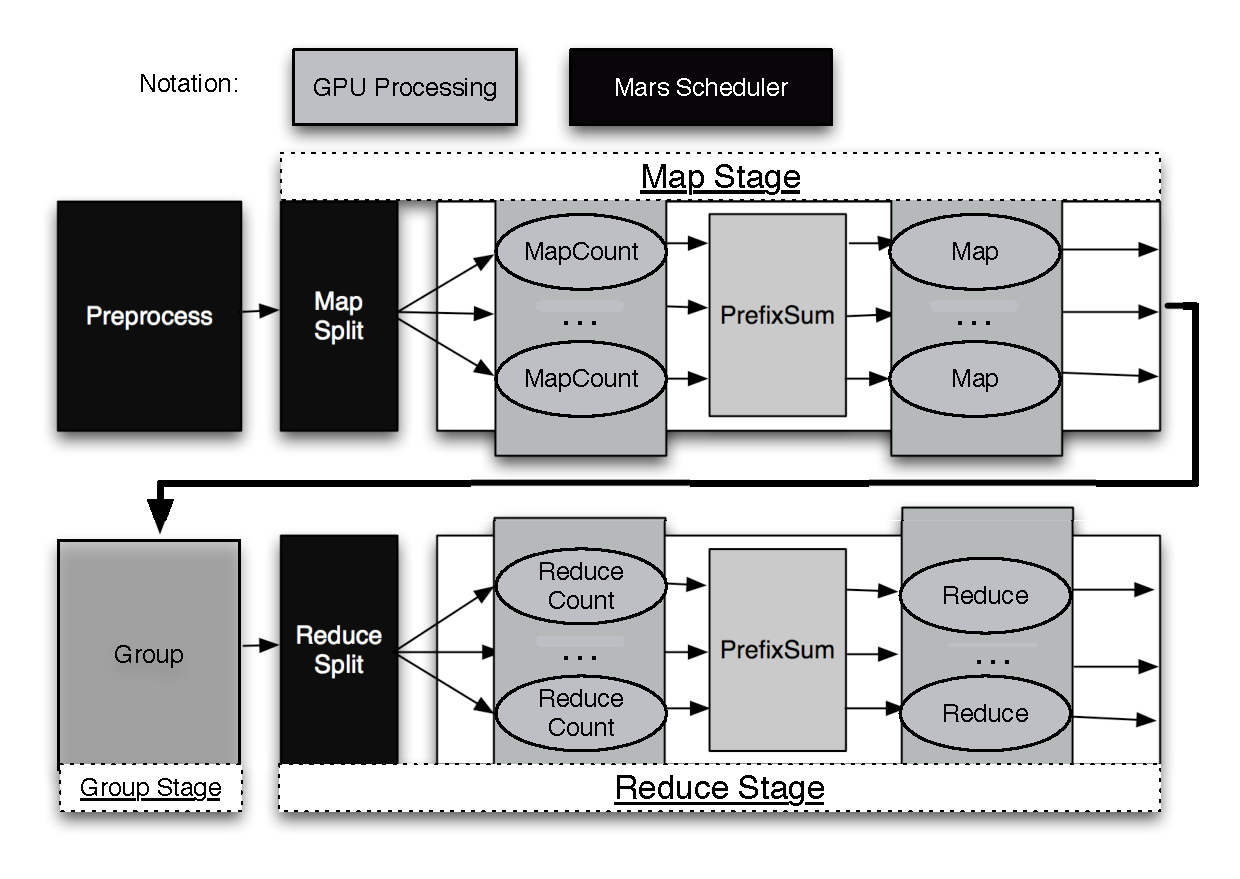
\includegraphics[width=0.60\textwidth]{figure/Mars_workflow.eps}
  \caption{The workflow of Mars on the GPU. }\label{fig:MarsWorkflow}
\end{figure}

{\em 1. Results on MarsBrook}



\doublerulesep 0.1pt
\begin{table}[htb]
  \centering
 \linespread{1.7}{ {\footnotesize
  \caption{Comparison on code sizes of MM and SS using MarsBrook and Brook+.}\label{tab:brookcodesize}
\vspace{2em}
  \begin{tabular}{ccc}
  \hline
\noalign{\smallskip}
  \textbf{Applications} & \textbf{MarsBrook} & \textbf{Brook+} \\
\noalign{\smallskip}
  \hline
  MM & 66 & 93 \\
  SS & 66 & 611  \\
  \hline
\noalign{\smallskip}
  \end{tabular}
  }}
\end{table}


\section{Research background and significance}

\textbf{Organization:} The remainder of the thesis is organized as
follows. We give a brief overview of GPUs, and review prior work on GPGPU and
MapReduce in Chapter~\ref{sec-preliminaries}. We present the design
and implementation details of Mars in Chapter~\ref{sec-design} and
Chapter~\ref{sec-implement} respectively. We present the extension
to multiple machines in
Chapter~\ref{sec-beyond}. In Chapter~\ref{sec-eval}, we present our
experimental results. Finally, we conclude in Chapter~\ref{sec-conclusion}.

\newpage
